\documentclass[]{article}
\usepackage{ listings} 
\usepackage{graphicx}
\graphicspath{ {images/} }
\usepackage{float}
\usepackage{geometry}
\usepackage{pdfpages}
\usepackage{multirow}

\usepackage{algorithm}  
\usepackage{algpseudocode}  
\usepackage{amsmath} 

\renewcommand{\algorithmicrequire}{\textbf{Input:}}
\renewcommand{\algorithmicensure}{\textbf{Output:}}

\makeatletter
\def\@maketitle{%       
	\newpage
	\null
	\vskip 14em%
	\begin{center}%
		\let \footnote \thanks
		{\LARGE \@title \par}%
		\vskip 12em%
		{\large
			\lineskip .5em%
			\begin{tabular}[t]{c}%
				\@author
			\end{tabular}\par}%
		\vskip 1em%
		{\large \@date}%
	\end{center}%
	\par
	\vskip 1.5em}
\makeatother
%opening
\title{\Huge COT5405 - Analys of Algorithms \\ Homework 1}
\author{Qinxuan Shi \\ UFID: 83518162}
\date{}
\special{papersize=8.5in,11in}
\geometry{left=2cm,right=2cm,top=1.5cm,bottom=1.5cm}

\begin{document}
	
	\maketitle
	\clearpage
	
	\section{Problem 1: Cycle finding}
	\subsection{Pseudo-code of the Algorithm}
		\begin{algorithm}  
			\caption{Cycle Finding}  
			\begin{algorithmic} 
				\Require $Graph\ G$  
				\Ensure
				\State Initially let \emph{\textbf{m}} be the number of edges of Graph \textbf{G}, and let \emph{\textbf{n}} be the number of vertices of Graph \textbf{G}
				\If{\emph{\textbf{m}} is greater than or equal to \emph{\textbf{n}}}
					\State There exist a cycle in \textbf{G}
				\Else
					\While{there exists vertex in the set of vertices of Graph G whose degree is less than or equal to 1}
						\State 1. Delete the vertex whose degree is less than or equal to 1, and delete the related edge
						\State 2. Minus the degrees of other vertices related to these edges by one
					\EndWhile

					\State \Return{the set \emph{\textbf{s}} of vertices after deletions}
					\If{there is no vertices in \emph{\textbf{s}}}
						\State There is no cycle in \textbf{G}
					\Else
						\State There exist a cycle in \textbf{G}
					\EndIf
				\EndIf
			\end{algorithmic}  
		\end{algorithm} 
		
	\subsection{Proof of the algorithm's correctness}
	
	To prove the correctness of the algorithm, it will be divided into two parts. The first part is to prove when the number of edges of Graph G is greater than or equal to the number of vertices of Graph G, there must be a cycle in G. The second part is to prove after the deletion is finished (which means there is no vertices in the set of vertices or there are still vertices in the set but their degrees are all greater than or equal to 2), if there are still vertices in the set, a cycle could be found in the Graph G.   \\
	
	\noindent Firstly, let's prove that when the number of edges of Graph G is greater than or equal to the number of vertices of Graph G, there must be a cycle in G. We can think from the direction of the spanning tree that each additional edge can connect two unconnected parts. At the beginning, there are n independent vertices, that is, n unconnected parts. After adding n-1 edges to get the spanning tree, the edges that continue to be added can only be in the connected parts. Therefore, at least n edges must form a loop (cycle). So, when the number of edges m is greater than or equal to the number of vertices n, there must be a cycle.  \\
	
	\noindent Secondly, we are going to prove if there are still vertices in the set after the deletion of vertices with degree less than or equal to 1, a cycle could be found in the Graph G. If there is a Cycle in Graph G, there must be a subgraph G', which is a Cycle. Degrees of all vertices in G' are greater than or equal to 2. We could consider this in another way. Now, we only have the graph G', which is a cycle, so it is clear that degree of each vertex of G' equals to 2. Then, we try to add edges and vertices to G' until it turns to the same graph as G. We can find out that during the process, no matter how many new edges and vertices are added, the degree of the vertices of G' will not decrease, which means the vertex V in G' will have at least two edges connected by other two vertices in G'. As a result, to the vertices in G, if there is a Cycle, assume that there is only one cycle, then after deleting all the vertices with degree less than 2, the subgraph G' will be left since all the vertices have 2 degrees. It is also the same when there are more than 1 cycle in the graph. So, we can know whether there is a cycle in the graph by checking if there are still vertices in the set after the deletion of vertices with degree less than or equal to 1.  \\
	
	\subsection{Algorithm's running time}
	
	According to the pseudo-code, to compare m and n, the complexity is clearly O(1).\\
	
	\noindent If m $\le$ n, we could divide the vertices less than or equal to 1 into two parts. The first part is vertices with degree 0, it is easy to figure out that delete a vertex with degree 0 only need 1 step (n times at most). The second part is vertices with degree 1, it is also clear that if you want to delete a vertex with degree 1, you need to delete an edge at the same time (delete edges are m times at most). The total number of these two operations will not exceed m + n, which means all the vertices plus all the edges. \\
	
	\noindent As a result, the total complexity is O(m + n).  \\
	
	\begin{figure}[H]
		\centering
		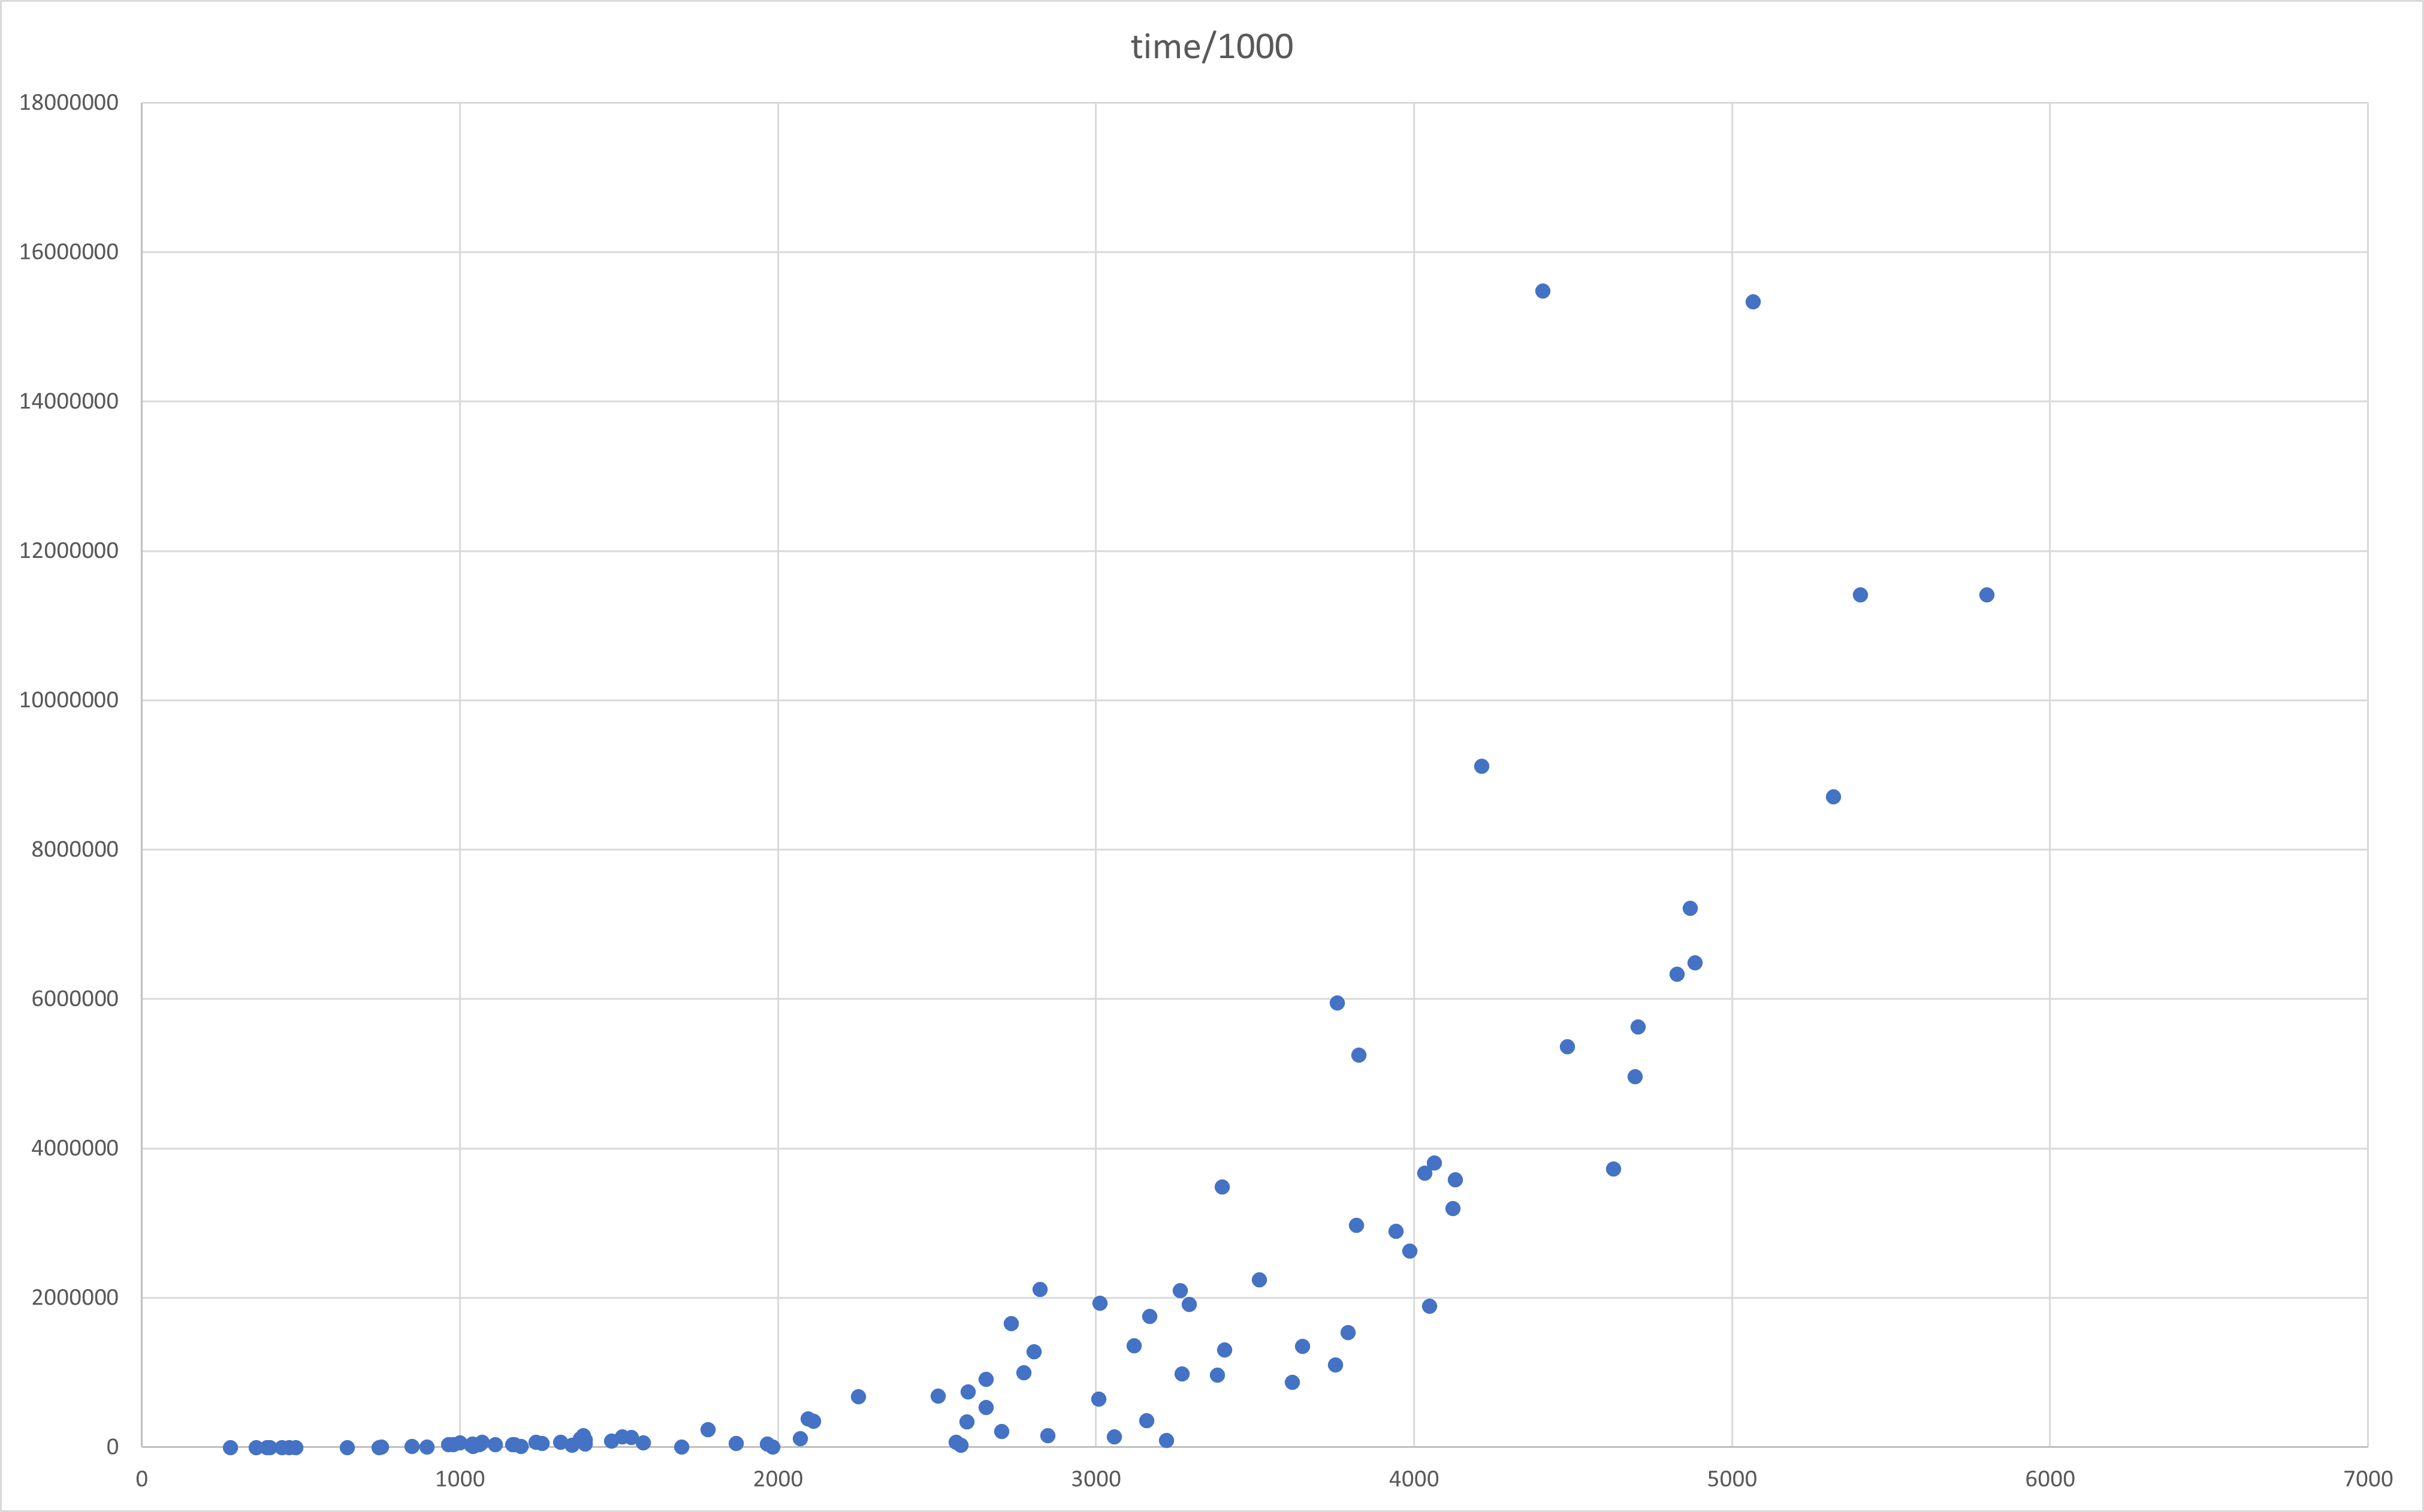
\includegraphics[width=0.9\linewidth]{screen/Picture1}
		\caption{function of size and running time}
		\label{fig:function-of-size-and-running-time}
	\end{figure}

	\begin{figure}[H]
		\centering
		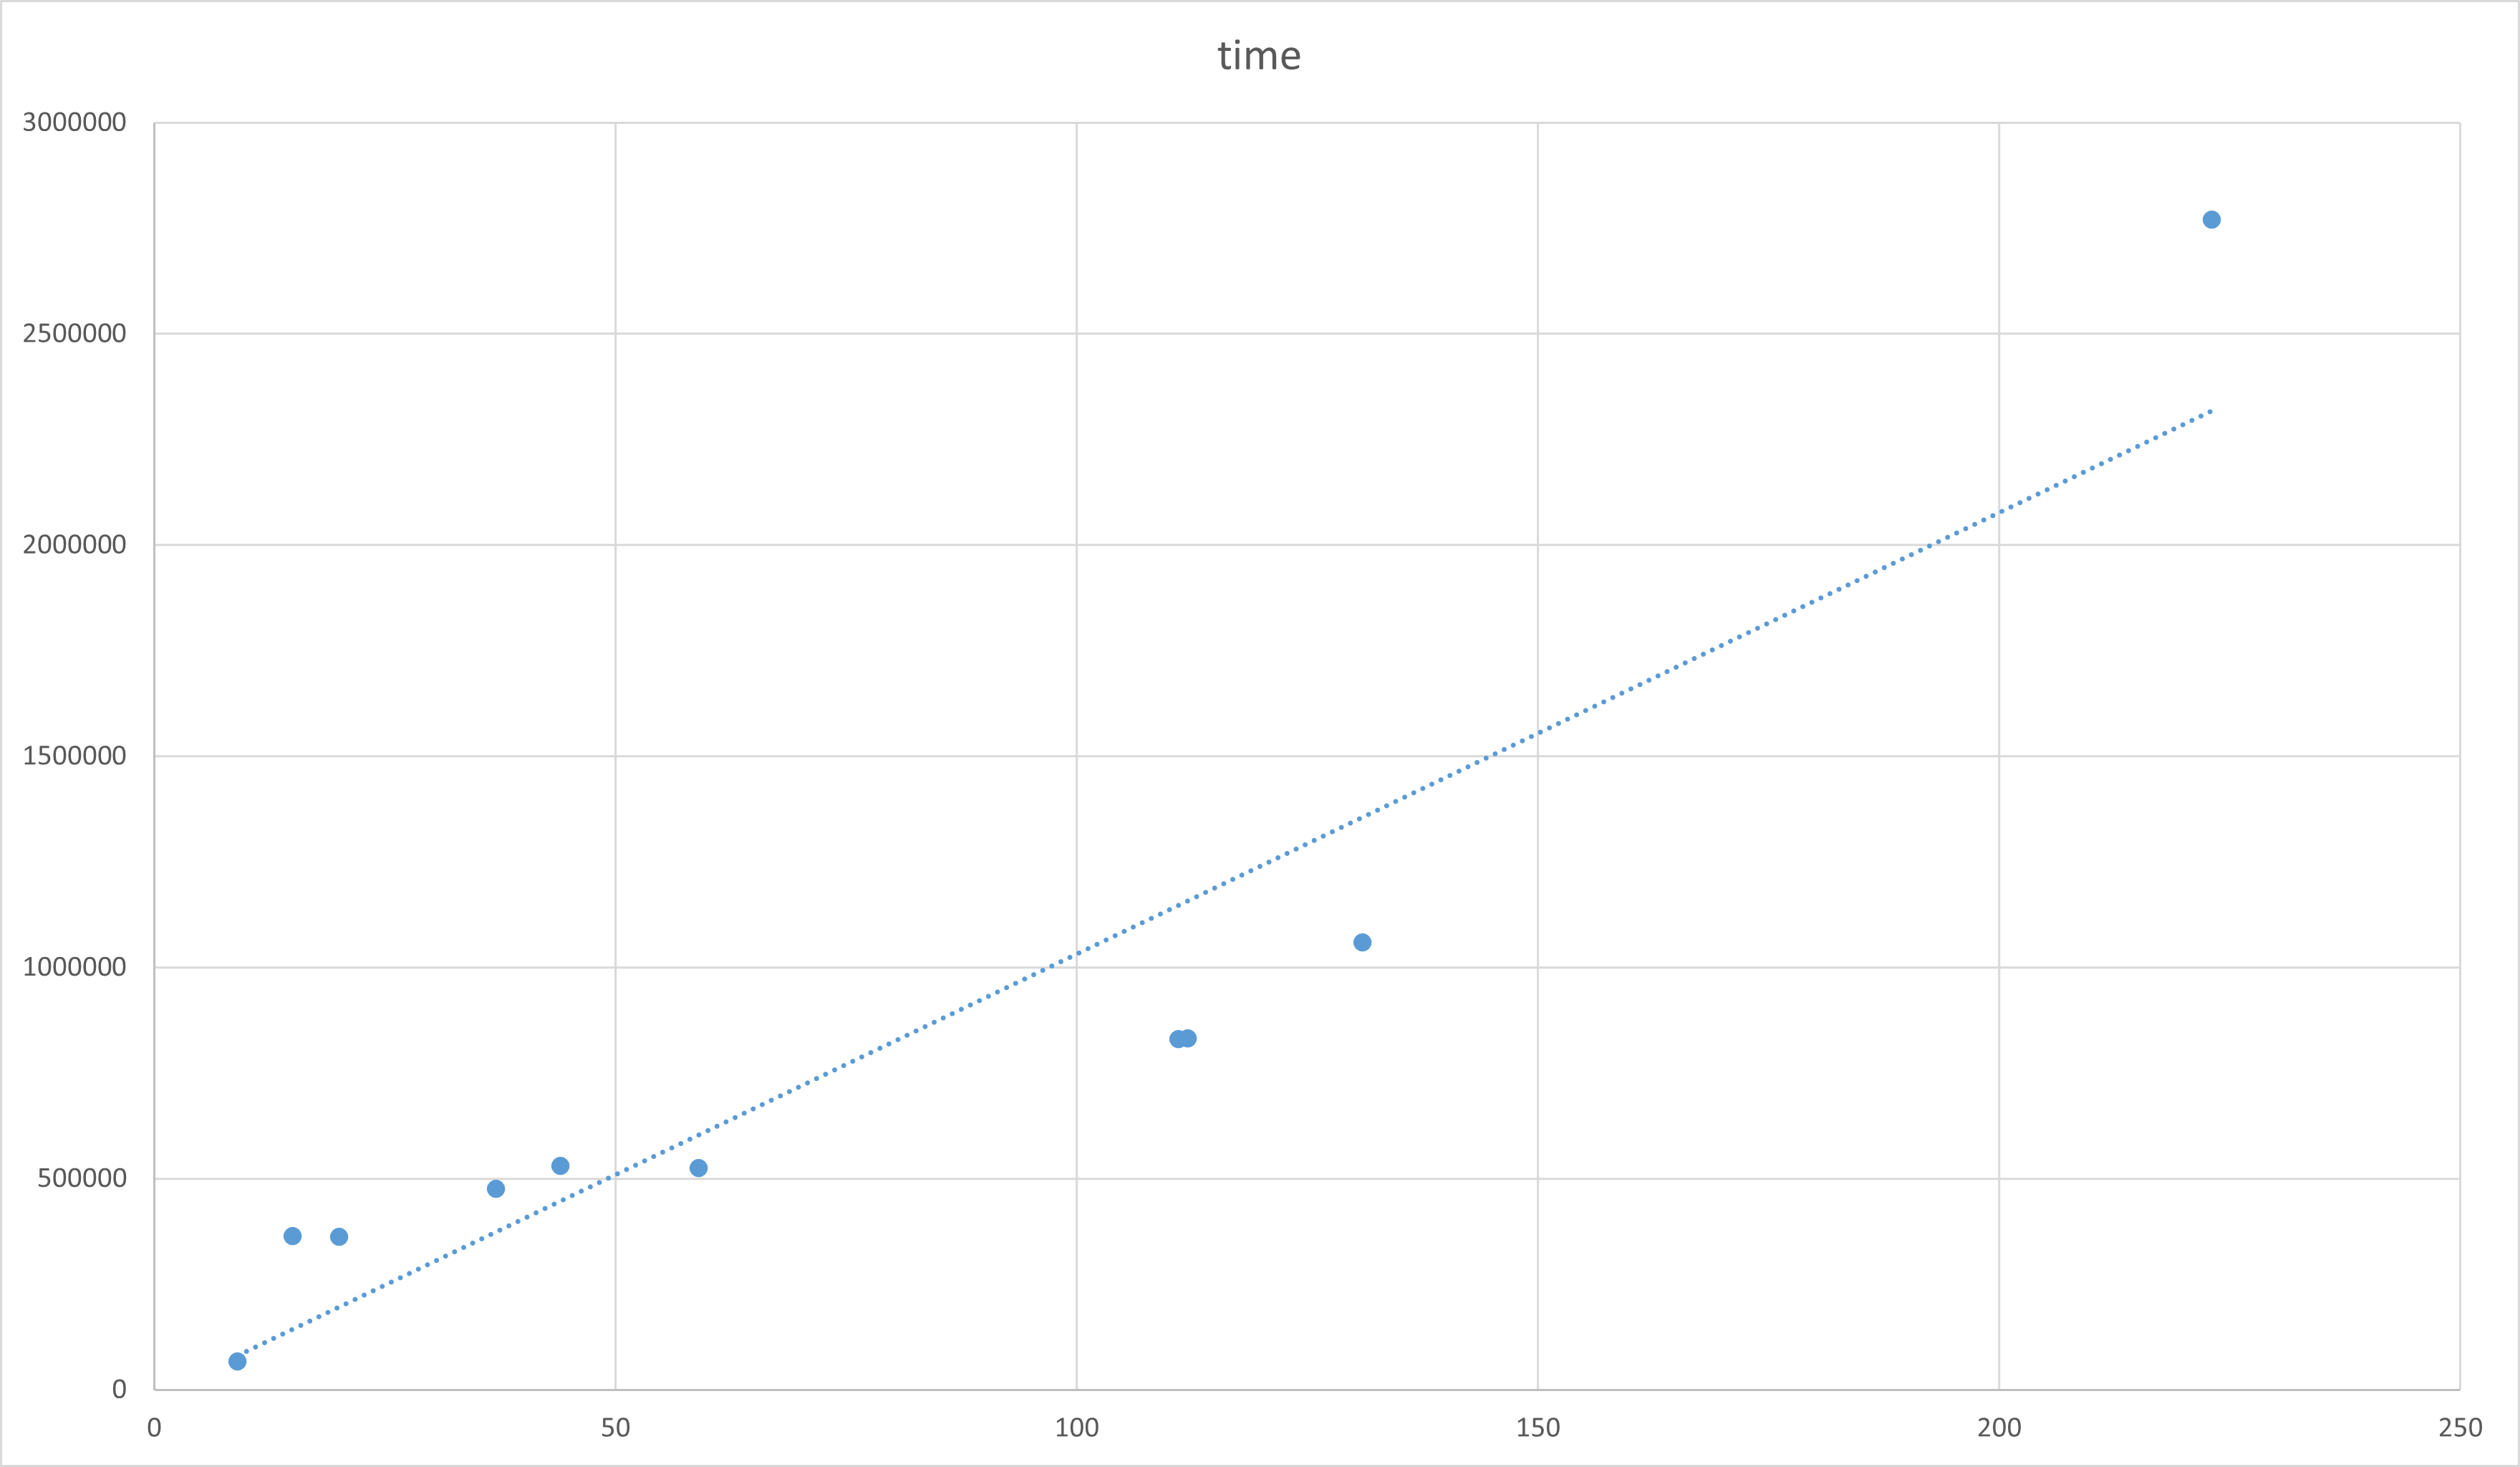
\includegraphics[width=0.9\linewidth]{screen/Picture2}
		\caption{Runningtime with small m + n}
		\label{fig:picture2}
	\end{figure}
	
	\noindent In Figure 1, I used 100 data pairs of records of running time, and the largest vertex number of the randomly generated graph is 3000. Besides, I do not take the situation that edge number is greater than or equal to vertex number into account, since the complexity of this situation is O(1), and if this kind of data are considered in the chart, it will be quite hard to figure out whether the running time is O(m + n). \\
	
	\noindent Here is the diagram that produced by using the excel to generate from the size of m plus n and running time. Since the time granularity is 2000000, so it is too large for the running time that is short. So when we start from the x-axis equals to 2500, and We can clearly figure out from the graph that after x-axis equals to 2500, these data could nearly form the function which is nearly linear. And it is the same for the x-axis less than 2000, which we could see clearly from Figure 2. So this is consistent with the analysis that the total complexity is O(m + n), which generally could also be seen as O(N). (Attention: Here we only consider the data which are all under the situation that $m \leq n$. Because when $m \geq n$, we can know that it takes O(1) to get the result, and these kinds of data is meaningless to be used to generate a diagram. Exactly, these kinds of data have the running time which fluctuate in a quite small range.)\\
	
	\clearpage
	
	\section{Problem 2: Minimum Spanning Tree for "sparse" graphs}
	\subsection{Pseudo-code of the Algorithm}
	\begin{algorithm}  
		\caption{Minimum Spanning Tree for "sparse" graphs}  
		\begin{algorithmic} 
			\Require $Graph\ G$  
			\Ensure
			\State Initially let \emph{\textbf{m}} be the number of edges of Graph \textbf{G}, and let \emph{\textbf{n}} be the number of vertices of Graph \textbf{G}, $w_{i}$ is the weight of the edge $i$.
			\If {Graph G is not connected}
			\State There is no spanning tree for Graph \textbf{G}
			\Else
			\State Firstly, we need to sort the edges according to their weight, and get the sorted edges set $S$.
			\For{i in set S}
				\If{G' already has $n-1$ edges}
					\State The Minimum Spanning Tree has been built
					\State Finish the loop
				\Else
				\State 1. Choose the edge $e[i]$ in S which has the smallest weight 
				\State 2. Add it to the graph G'(G' is an empty graph at the begining)
				\State 3. Check out if the graph G' has a loop after adding $e[i]$
				\If{G' has a loop}
					\State Do not add $e[i]$, consider the next edge $e[i+1]$ which is equal to or only smaller than $e[i]$
				\EndIf
				\EndIf
			\EndFor
			\EndIf
		\end{algorithmic}  
	\end{algorithm} 
	
	\subsection{Proof of the algorithm's correctness}
	
	To prove the algorithm's correctness, we need to prove two parts, the first part is the correctness of algorithm used to check if the graph is connected and the second part is to prove that the algorithm finds a minimum spanning tree.  \\
	
	\noindent Firstly, we are going to prove the correctness of connection algorithm. I used the DFS to traverse the graph G start from the vertex 0, and here I have a parameter 'count' to get the number of vertexes that have been visited by the algorithm. For the reason that if the graph G is connected, there is a path between each pair of $[v_{i},v_{j}]$. This algorithm does not try to get every vertex, it only traverse from one vertex to check that if there is a road to each of the other vertexes. So we only need to compare the number of vetexes to count, if they are equal, then the graph is connected.   \\
	
	\noindent Then, we will prove the correctness of the algorithm that is used to find the minimum spanning tree.  \\
	
	\noindent 1. The algorithm can get a spanning tree. \\
	
	\noindent Assuming that the algorithm does not get a spanning tree, according to the definition of the tree, there are two cases: the first case is that the graph has loop, and the second case is that the graph is not connected. Since the algorithm check if there is a loop in the new generated graph G' every time when new edge added to graph G', so there couldn't be any loop in the graph. To the second case, since the algorithm stops when there are $n-1$ edges added to the graph G' and the graph G' does not have a cycle, it's impossible for G' to be unconnected. As a result, the algorithm can get a spanning tree.   \\
	
	\noindent 2. The spanning tree get from the algorithm is a minimum spanning tree. \\
	
	\noindent We assume that the tree gets from the algorithm T is not the minimum spanning tree, so there must be a minimum spanning tree, we call it $T_{1}$. So, there must be one step makes T has greater toatl weight then $T_{1}$. However, to the tree T, other edges that haven't been added to the graph G' all have larger weight than the edge that has just been added to the tree T. For each step, there won't be any other tree that will have less total weight than T. Exactly, the algorithm is a greedy algorithm, it gets the optimal choice for each step. As a result, the spanning tree get from the algorithm is a minimum spanning tree. \\
	
	\subsection{Algorithm's running time}
	According to the pseudo-code, if we want to compute the complexity of the Algorithm, we need to consider three parts.\\
	
	\noindent The first part is to check out whether the graph is connected. Here, I use the DFS to traverse the graph G, and get the result. The complexity of DFS by using adjacency matrix is O($n^{2}$). \\
	
	\noindent The second part is to sort the list of edges according to their weight. Exactly, there are several kinds of ways to sort and I userd Insertion Sort, since the sort has two for-loops, it is also clear that the complexity is O($n^{2}$).  \\
	
	\noindent The last part is complexity of the for-loop. For the reason that the graph G is a sparse graph and its edge is no more than $n+8$, so the loop will run at most $n+8$ times, the action of add is O(1), but the complexity of finding a loop is O(m+n), which is proved in section 1. As a result, the complexity of part three is also O($n^{2}$).\\
	
	\noindent To conclude, the total complexity is O($N^{2}$).  \\
	
	\begin{figure}[H]
		\centering
		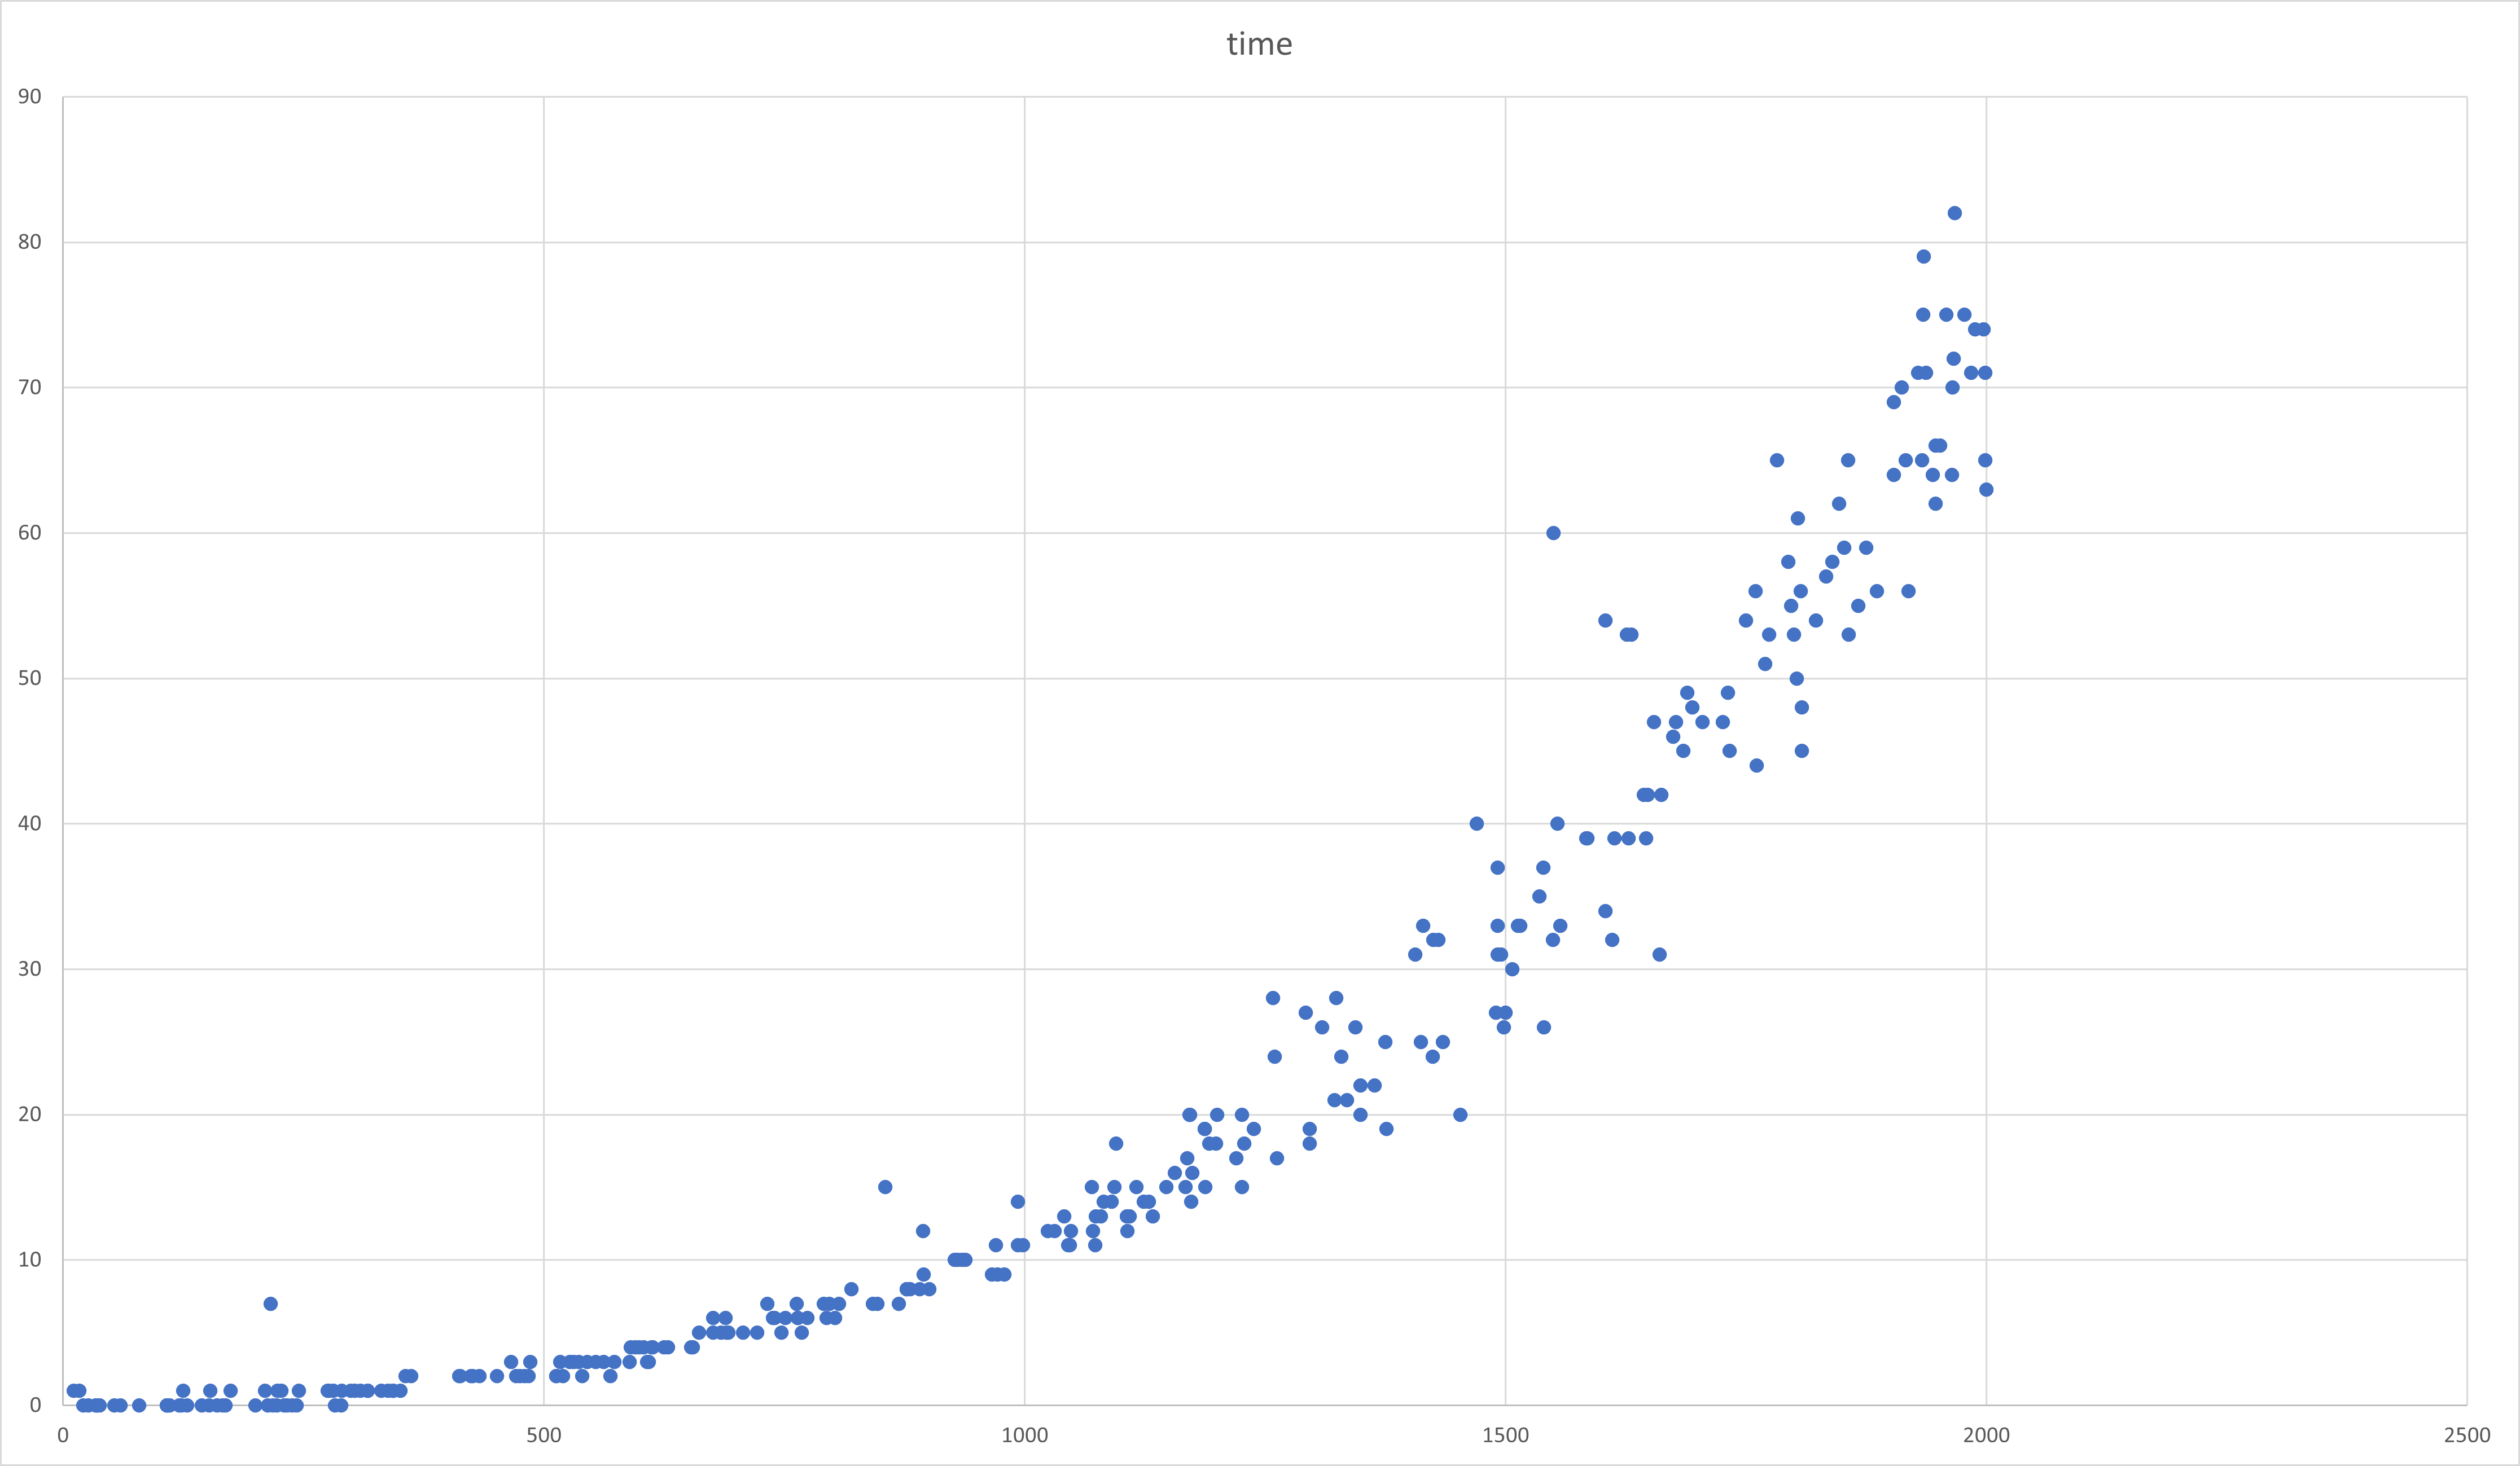
\includegraphics[width=1.0\linewidth]{screen/Picture3}
		\caption{Assignment2 running time}
		\label{fig:function-of-size-and-running-time}
	\end{figure}
	
	\noindent In Figure 3, I use 300 data pairs of records of running time, and the largest vertex number of the randomly generated graph is 2000. Because of the reason that it is quite easy to generate unconnected graph which also has the number of edge m that m fulfills $m\in[n-1,n+8]$, I try to record more data in order to get enough right data to build a diagram. \\
	
	\noindent Here is the diagram that produced by using the excel to generate from the number of n and running time. It is clear to figure out that the pairs of data could forms the function which is similar to $y=n^{2}$.\\
	
	\clearpage
	
\end{document}
\documentclass[]{article}

%opening
\title{}
\author{}

\begin{document}

\maketitle

\begin{abstract}

\end{abstract}

\section{}

\end{document}
